\documentclass[12pt,longbibliography]{article}
\usepackage[utf8]{inputenc}
\usepackage[T1]{fontenc}
\usepackage[catalan]{babel}
\usepackage[a4paper, margin=2.7cm]{geometry}

\usepackage{amsmath, amsthm, amsfonts, amssymb}
\newtheorem{thm}{Theorem}[section]
\newtheorem{cor}[thm]{Corollary}
\newtheorem{lem}[thm]{Lemma}
\newtheorem{prop}[thm]{Proposition}
\theoremstyle{definition}
\newtheorem{defn}[thm]{Definition}
\theoremstyle{remark}
\newtheorem{rem}[thm]{Remark}

\usepackage{mathrsfs} 
\usepackage[colorlinks=true,linkcolor=blue,citecolor=blue,urlcolor=blue,breaklinks]{hyperref}

\usepackage{bbm} 

\usepackage{hyperref}
\usepackage{graphicx}
\graphicspath{ {Imatges portada/} }

\title{Big Query}
\author{Anna Salazar}

\renewcommand{\contentsname}{Índex}
\renewcommand{\figurename}{Figura}
\renewcommand{\tablename}{Taula}

\begin{document}
\begin{titlepage}
\maketitle

\vspace{140mm}

\par
\raisebox{-.5\height}{
\includegraphics[width=6cm]{fme}}%
\hfill
\raisebox{-.5\height}{
\includegraphics[width=6cm]{UB}}%
\par

\end{titlepage}

\tableofcontents

\pagebreak

\pagenumbering{arabic}

\section{Què és BigQuery?}

BigQuery és un motor d’anàlisi de macrodades (Big Data) que permet executar consultes SQL al núvol sobre les dades emmagatzemades en aquest, sense importar el volum de les dades ni el tipus de consultes que es volen fer. El motor de consulta és capaç de treballar sobre terabytes de dades en qüestió de segons, i sobre petabytes en pocs minuts. Avui en dia, les empreses estan adoptant cada cop més la presa de decisions basades en dades i fomentant una cultura oberta en la qual les dades no estan aïllades dins dels departaments. BigQuery, en proporcionar els mitjans tecnològics per a promoure un canvi cultural cap a l’agilitat i l’obertura, realitza un paper molt important en l’augment del ritme de la innovació.

\vspace{2mm}

Treballar amb dades a BigQuery implica 3 aspectes principals: l’emmagatzemament, la incorporació de les dades i la consulta d’aquestes, Google s’encarrega de tota la resta. Com BigQuery és un servei totalment gestionat, no és necessari configurar ni instal·lar res en el nostre ordinador i, pel mateix motiu, no necessitem un administrador de la base de dades. Simplement, podem entrar en el nostre projecte de Google Cloud des del nostre navegador i començar a analitzar.

\vspace{2mm}

Pel que fa a l’emmagatzemament, les dades es guarden en una taula estructurada, la qual cosa significa que es pot utilitzar l’SQL estàndard per a facilitar la consulta i l’anàlisi de dades. BigQuery és perfecta pel Big Data perquè gestiona tot aquest emmagatzemament i està proveïda d’operacions d’escalabilitat que funcionen de forma automàtica sense que l’usuari s’hagi d’involucrar,  per la qual cosa mai haurem de preocupar-nos per la grandària de les dades amb els quals treballem. Part de la consideració de disseny darrere de BigQuery és animar als usuaris a centrar-se en els coneixements en lloc de la infraestructura. Quan s’introdueixen les dades a BigQuery no és necessari pensar en els diferents tipus d’emmagatzemament, ni en els seus avantatges pel que fa a velocitat i cost; l’emmagatzemament està totalment gestionat.

\vspace{2mm}
\noindent
Per a més informació sobre BigQuery, es pot consultar la pàgina de \href{https://cloud.google.com/bigquery/docs/introduction}{Google Cloud}.

\subsection{Per què hauríem d'utilitzar BigQuery en lloc d'altres eines?}

Una de les característiques més rellevants que presenta BigQuery és que es tracta d'una plataforma sense servidor, és a dir, que els servidors s'executen en segon pla, sense l'intervenció de l'usuari. A més, presenta una alta disponibilitat, la qual cosa es tradueix en que no cal preocupar-se per la caiguda dels servidors, ja que la plataforma s'encarrega d'això. Per últim, BigQuery també té propietats d'escalabilitat automàtica que fan possible gestionar fins a petabytes de dades. Aquestes característiques no estan disponibles a la majoria de plataformes d'emmagatzament de dades tradicionals, cosa que fa destacar BigQuery entre moltes.

\vspace{2mm}

Com en molts altres magatzems de dades, BigQuery és capaç de treballar amb moltes fonts de dades diferents. Podem pujar les dades des del nostre propi sistema d'arxius, de Google Cloud Storage, de Google Drive i de moltes fonts més. Després de fer-ho, es poden consultar aquestes dades utilitzant SQL estàndard o SQL heretat, el rendiment en qualsevol cas és excel·lent. Els resultats de les consultes solen emmagatzemar-se en la memòria cau durant 24 hores, de manera que les següents execucions d'aquesta consulta només hauran d'obtenir les dades de la memòria cau en lloc de fer-ho del disc. 


\pagebreak

\section{Creació i treball amb conjunts de dades i taules}

\subsection{Configuració de la Plataforma de Google Cloud (GCP)}

\graphicspath{ {BigQuery/Imatges tutorial/} }

Per utilitzar aquesta eina d’anàlisi només ens caldrà crear un compte a Google Cloud i treballar a la zona de proves que ofereix Google per treballar de forma gratuïta.
Per fer servir la zona de proves (\textit{Sandbox}) seguirem els passos següents: 

1. En primer lloc, ens dirigim a la interfície d’usuari de \href{https://console.cloud.google.com}{BigQuery}. Des d'aquesta interfície es poden realitzar la majoria de les operacions.

\vspace{2mm}

2. Accedim al nostre compte de Google o creem un nou compte si encara no en tenim cap. Si és el primer cop que iniciem sessió a Google Cloud, haurem de marcar el país on som i acceptar les condicions de servei.

\vspace{2mm}

3. Un cop dins, podem veure com és l'espai de treball SQL. Hi ha una secció de l'Explorador a l'esquerra que ens permet navegar en projectes, conjunts de dades i taules.Per tal de fer servir la zona de proves, haurem de crear un projecte.

Introdueix un nom al teu projecte i fes clic a Create. En el nostre cas, hem anomenat el projecte \verb|el_meu_projecte|, i treballarem sobre aquest per il·lustrar el funcionament de la plataforma.
\vspace{2mm}
\par
\raisebox{-.5\height}{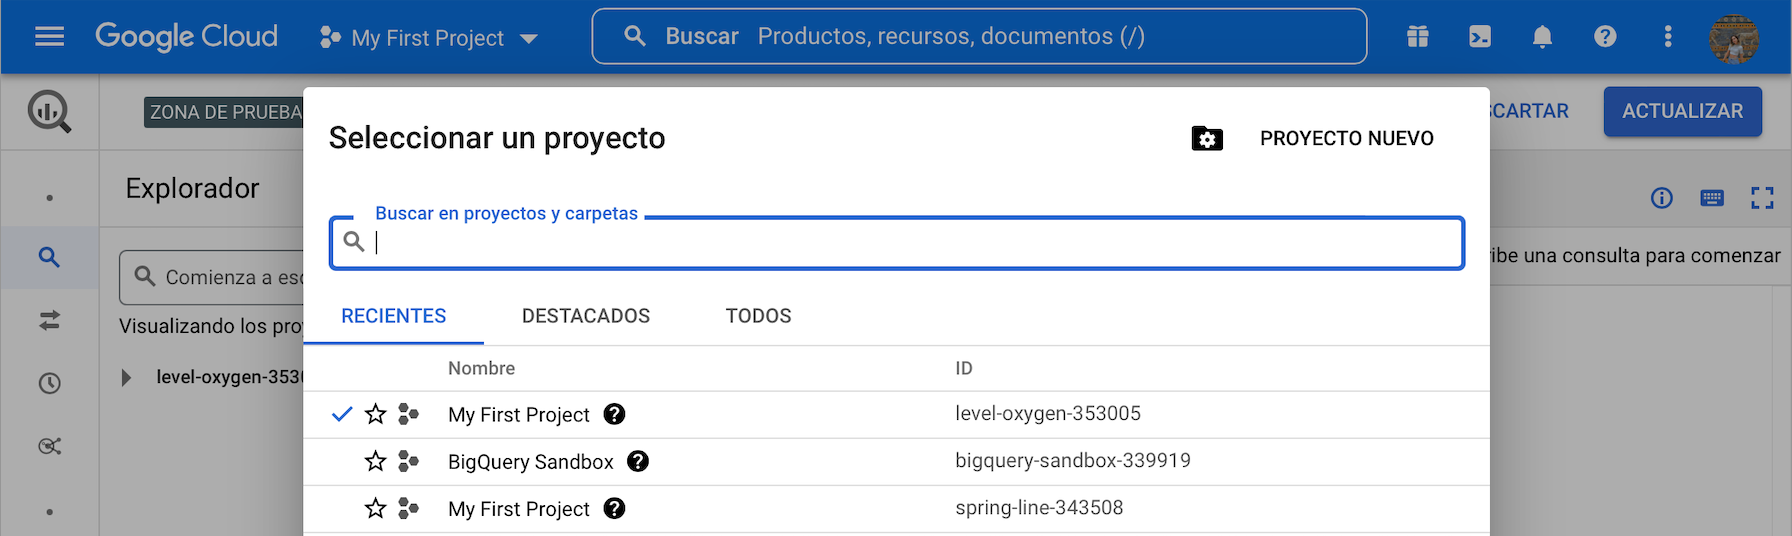
\includegraphics[width=7.25cm]{bq1}}%
\hfill
\raisebox{-.5\height}{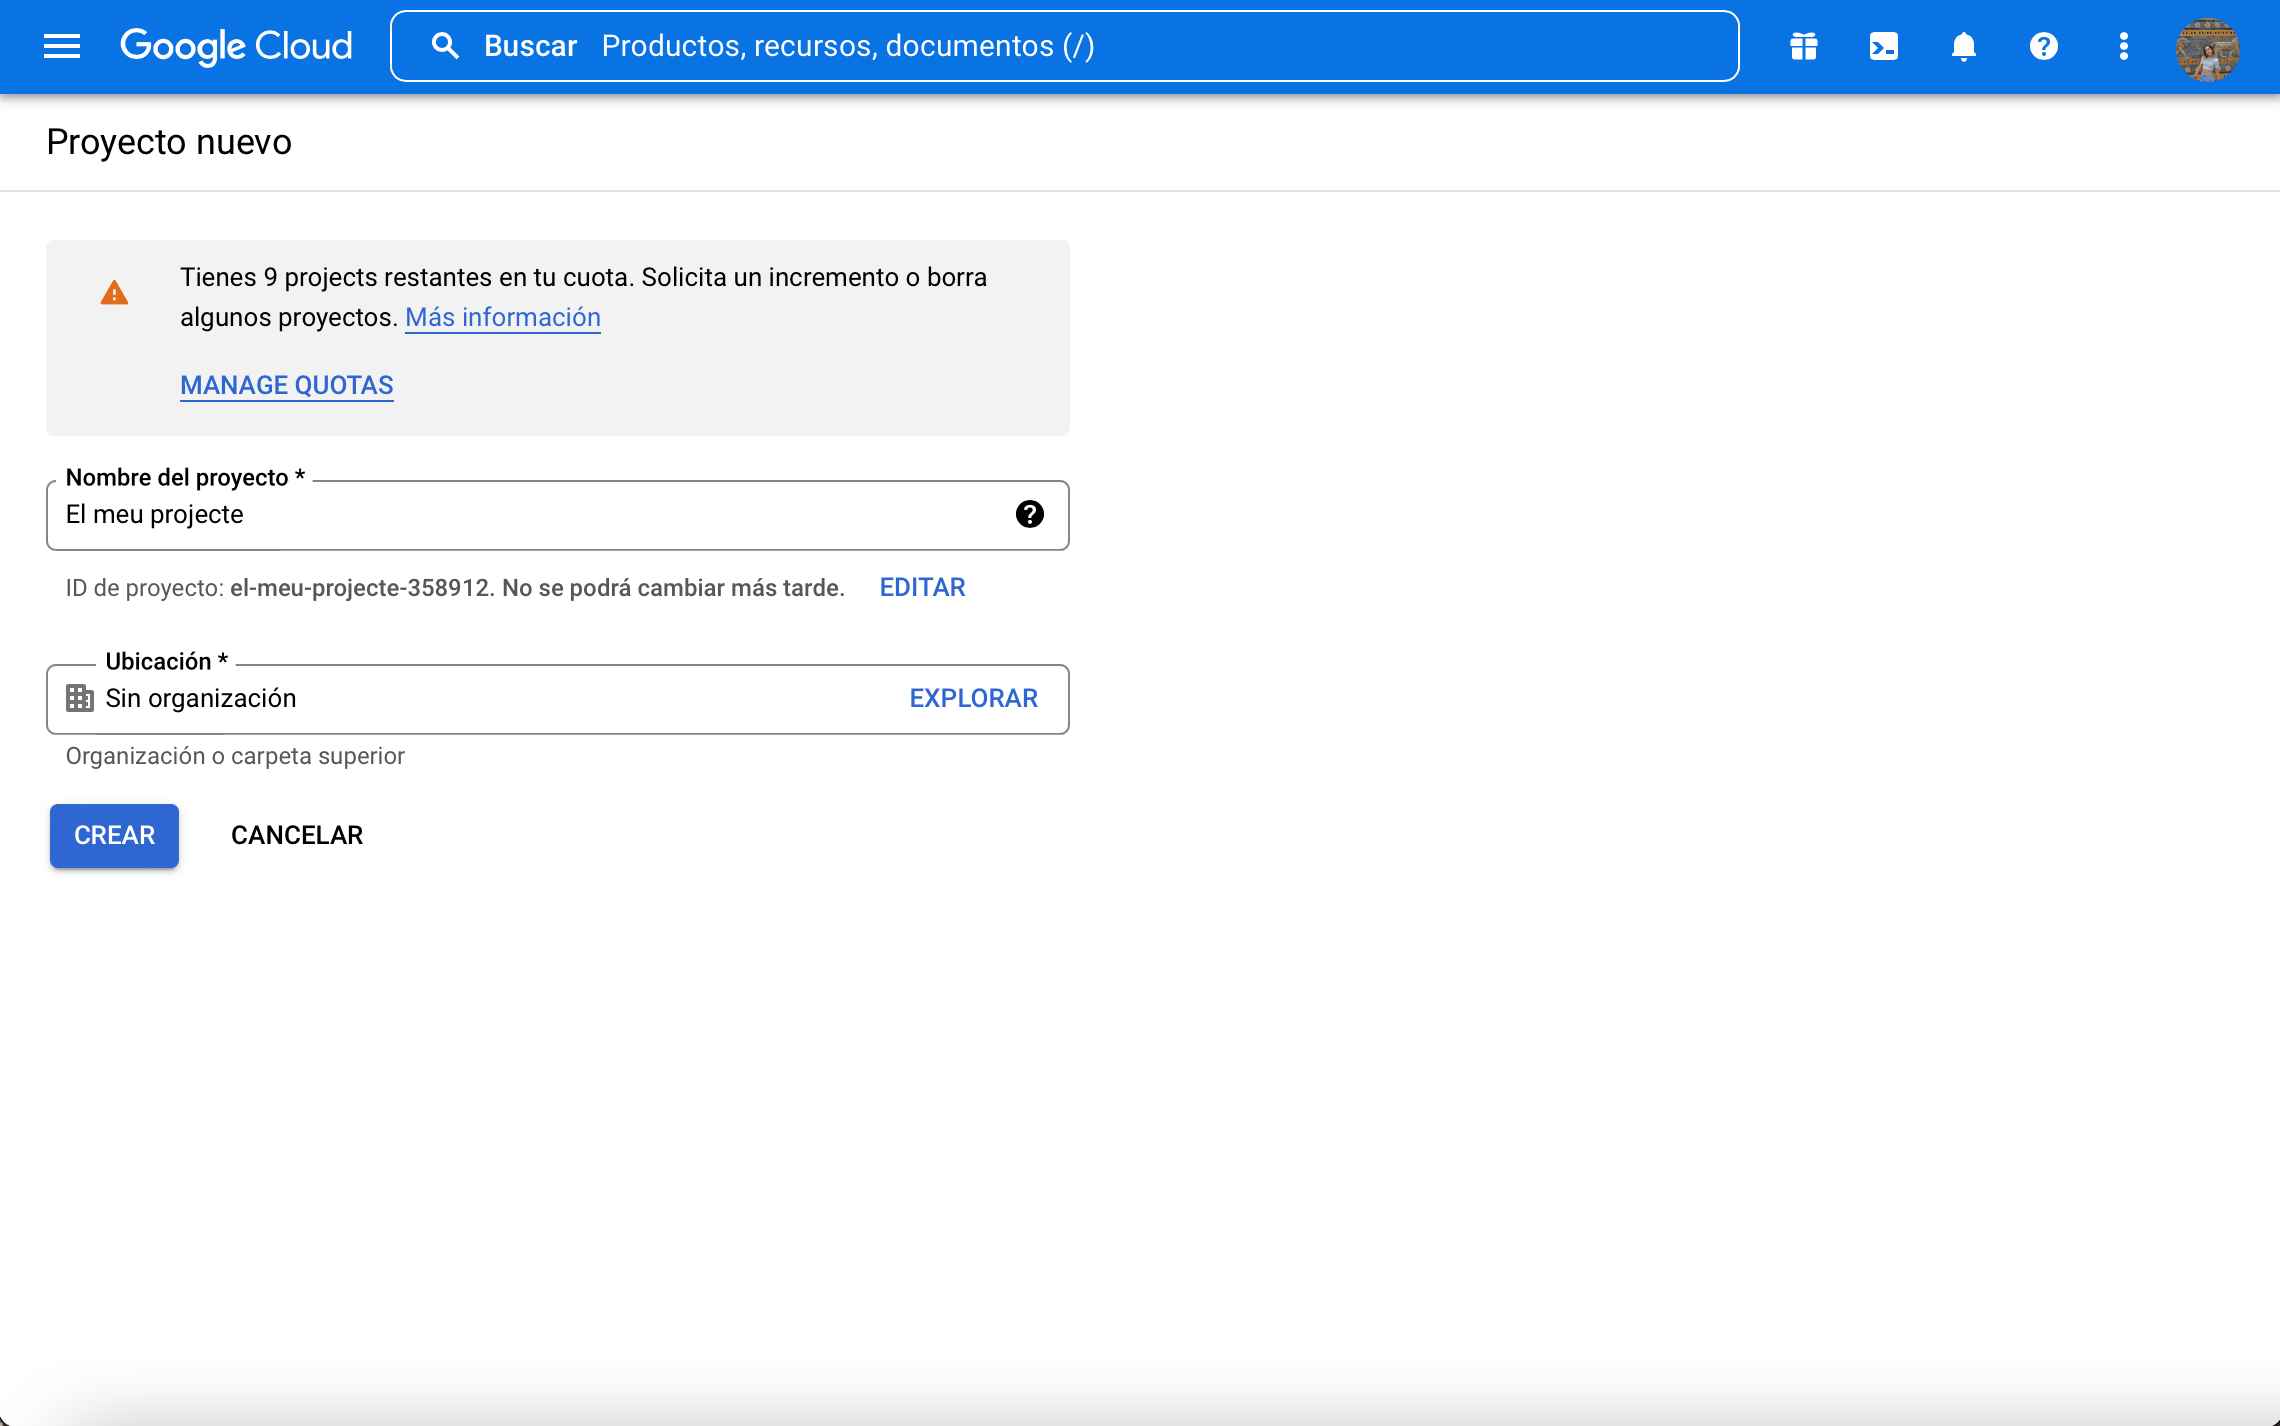
\includegraphics[width=7.25cm]{bq2}}%
\par
\vspace{2mm}
4. Un cop creat el projecte, el navegador ens redirigigeix a la interfície web de BigQuery.

\vspace{2mm}

5. Ara ja podrem carregar o consultar dades en el nostre projecte sense cap compte de facturació adjunta.

\subsubsection{Limitacions}

Per a l’ús de la zona de proves gratuïta que ofereix Google, haurem de tenir en compte un seguit de limitacions.

\vspace{2mm}

En primer lloc, ens trobem amb un màxim de 10 Gb d’emmagatzemament i 10 Tb de consulta al mes. Al llarg d’aquest projecte no utilitzarem un volum de dades més gran ni sobrepassarem el límit d’espai de consulta, però s’han de tenir en compte aquestes limitacions si l’objectiu és treballar amb el format gratuït.

\vspace{2mm}

A més, ens trobem que tots els conjunts de dades tenen el temps de caducitat de la taula per defecte establerta en 60 dies. Per tant, totes les taules, vistes o particions de les taules caducaran automàticament passats els 60 dies.

\vspace{2mm}

Una altra característica destacable és que els projectes de la zona de proves no són compatibles amb:

- La transmissió de dades

- Sentència de llenguatge de manipulació de dades (DML)

- Servei de transferència de dades de BigQuery

\subsection{Creació d'un conjunt de dades}

Ara que ja coneixem les limitacions de la plataforma i disposem d'un projecte en el que crear un conjunt de dades, ha arribat el moment de crear un nou conjunt de dades dins d'un projecte. Es pot pensar en un conjunt de dades a \textit{BigQuery} com una agrupació lògica de taules. Alhora, diferents cojunts de dades s'integren en un mateix projecte. 

\vspace{2mm}

Per a crear-ne un, només s'ha de desplegar el menú i triar l'opció de crear un nou conjunt de dades. Tot seguit hi ha diversos detalls per al conjunt de dades que es poden establir. En primer lloc, hi ha l'opció de canviar el projecte que l'encabirà. Això farà que aparegui un navegador on es pot especificar el projecte. Una altra possibilitat serà escollir la ubicació de les dades. Això determina on s'aprovisionaran els recursos subjacents, com la computació i l'emmagatzematge, per al servei \textit{BigQuery}. Les consideracions a l'hora de triar una ubicació inclouran el rendiment per als usuaris finals, l'alta disponibilitat i també qualsevol restricció d'auditoria o compliment. I, per últim, es pot establir un temps d'expiració per defecte per a les taules dins d'un conjunt de dades.

\vspace{2mm}

\par
\raisebox{-.5\height}{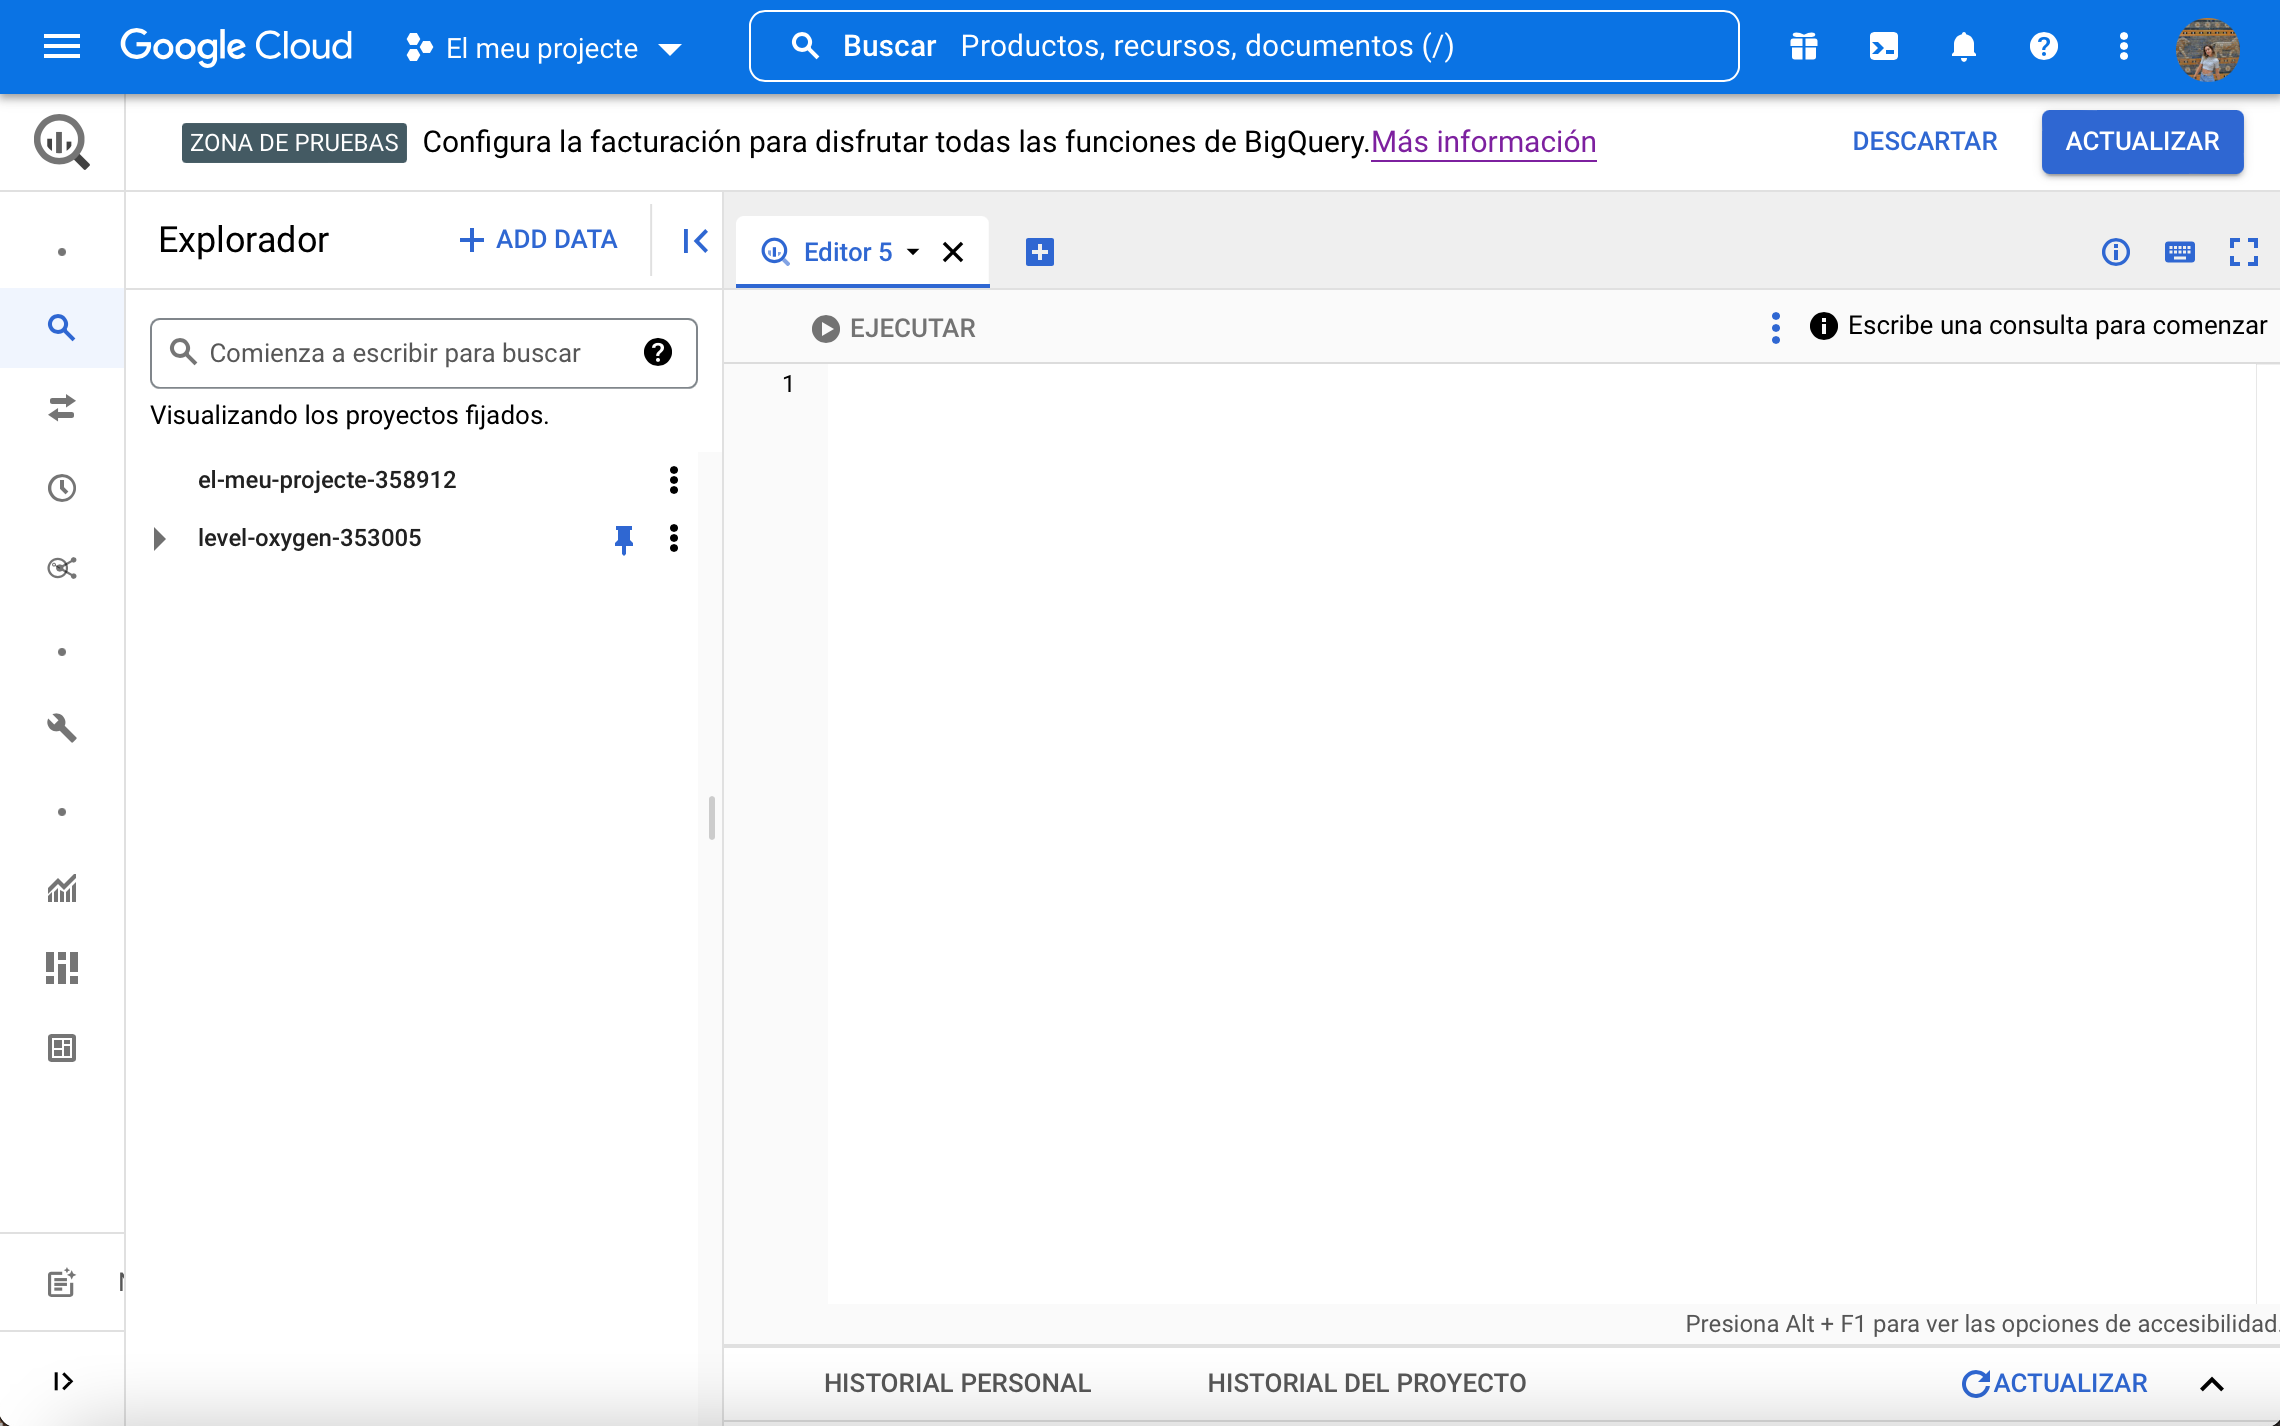
\includegraphics[width=7.25cm]{bq3}}%
\hfill
\raisebox{-.5\height}{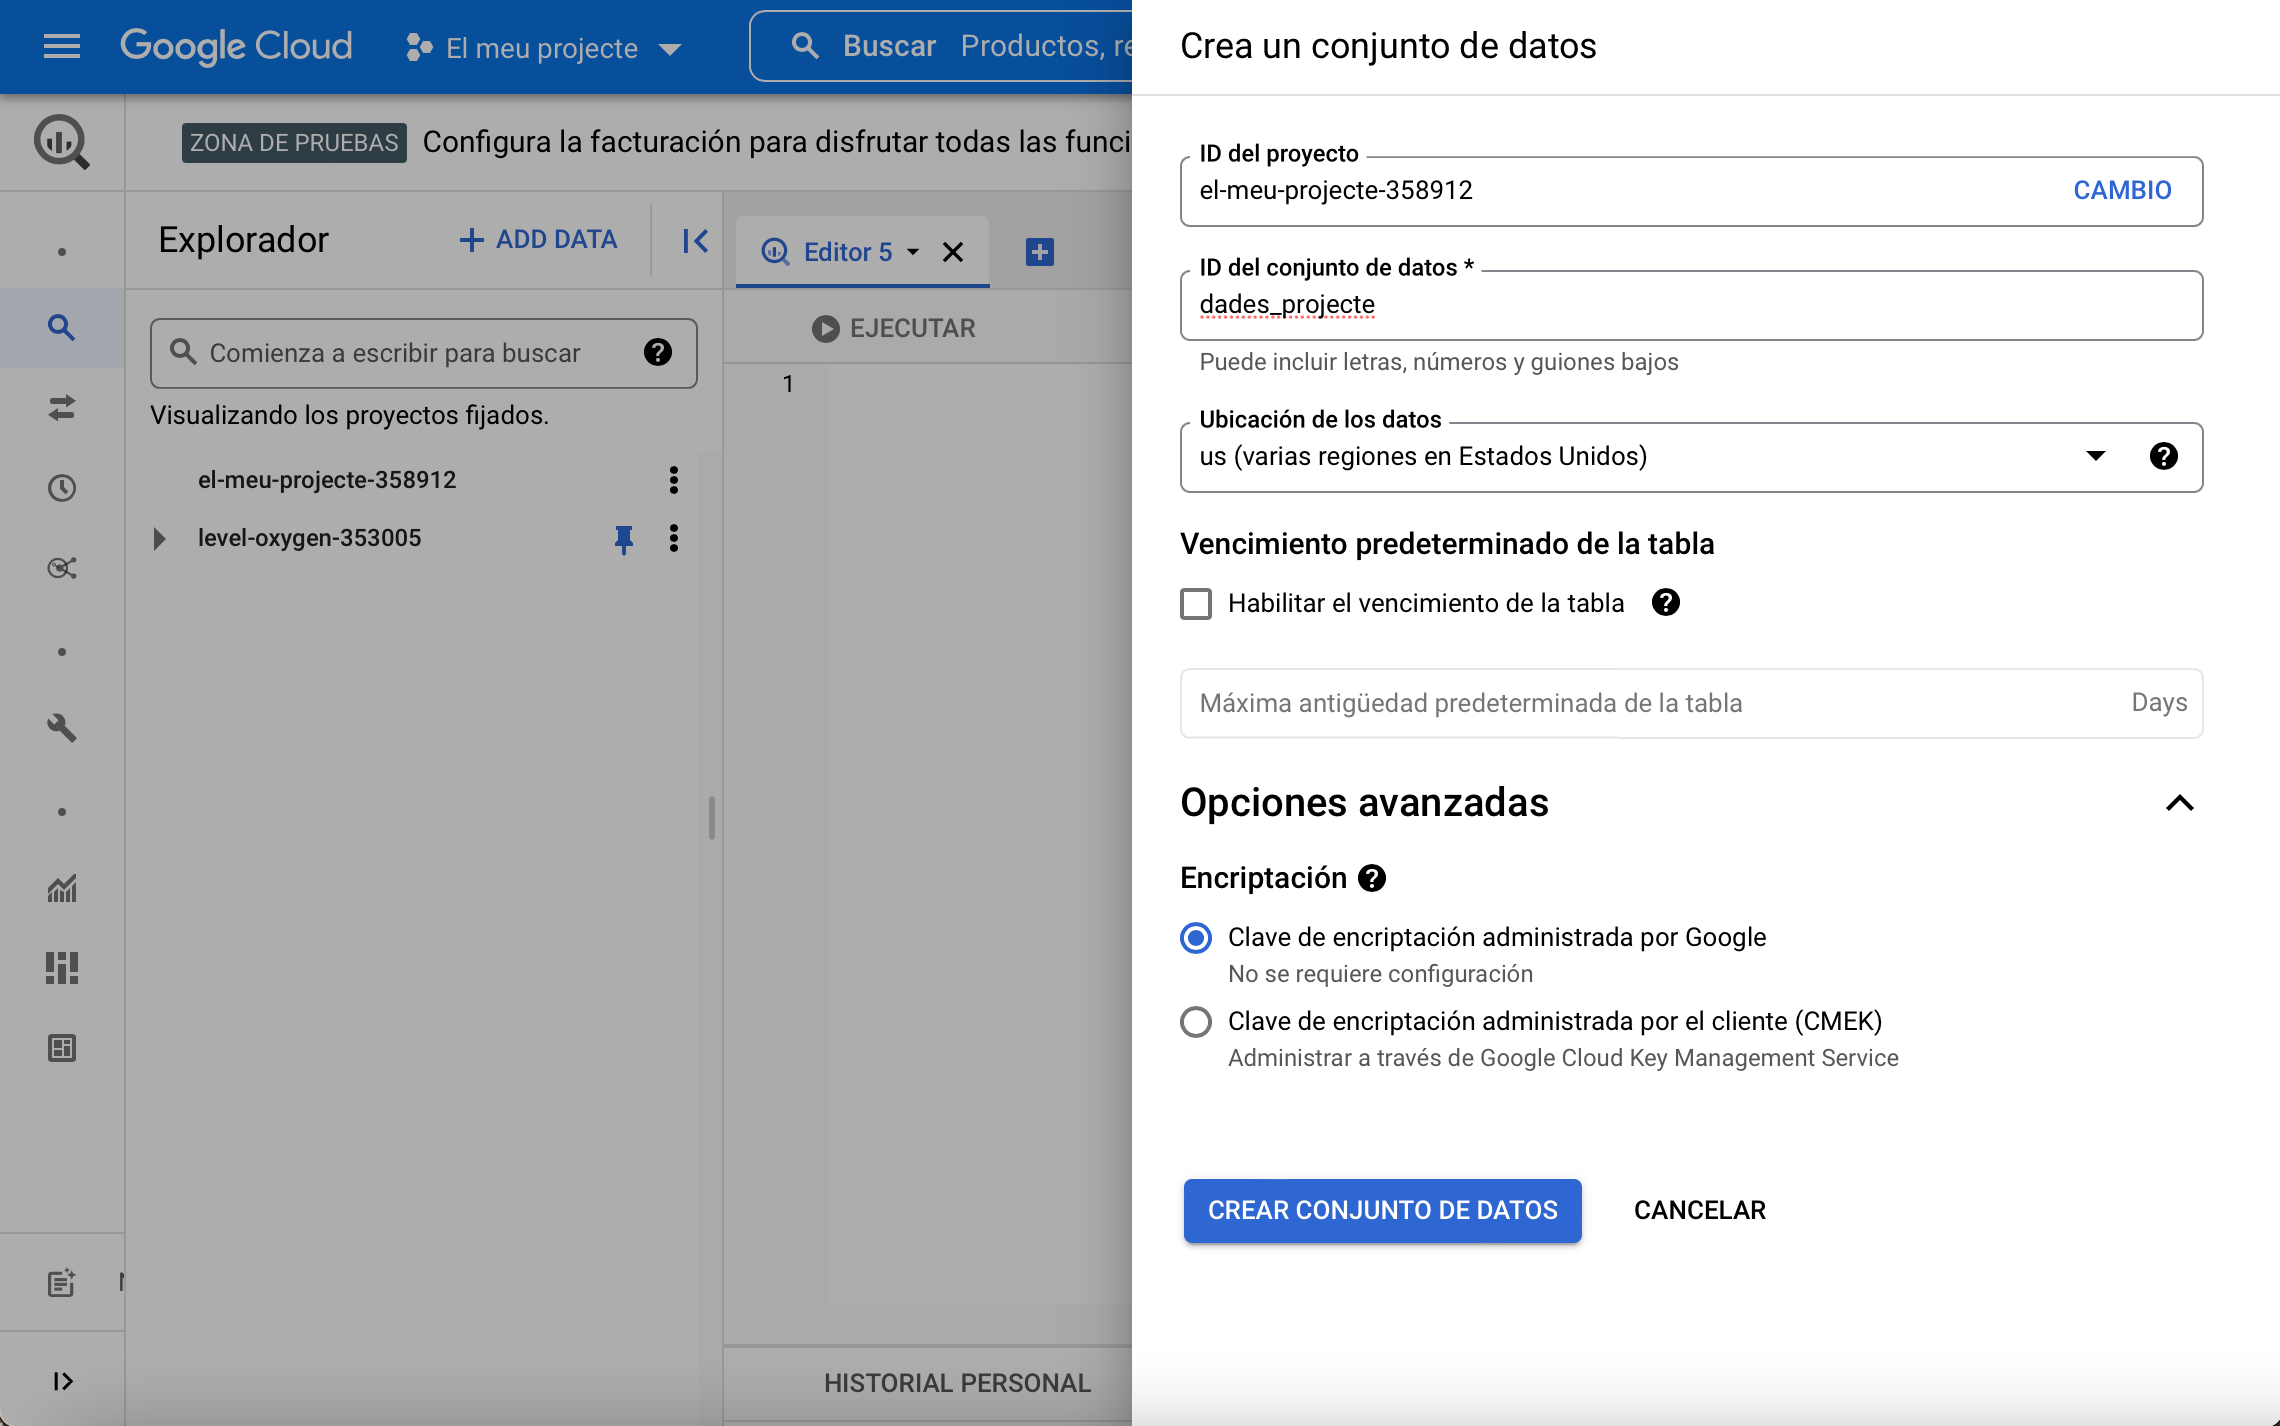
\includegraphics[width=7.25cm]{bq4}}%
\par

\vspace{2mm}

Tal com es pot veure a la figura anterior, hem creat un nou conjunt de dades anomenat \verb|dades_projecte| que estarà ubicat en el projecte \verb|el_meu_projecte|, la ubicació de les dades la hem posat a diverses regions dels Estats Units i, per últim, no hem habilitat un temps de venciment de la taula, sinó que per defecte \textit{BigQuery} l'emmagatzemarà per 60 dies.

\vspace{2mm}

\begin{center}
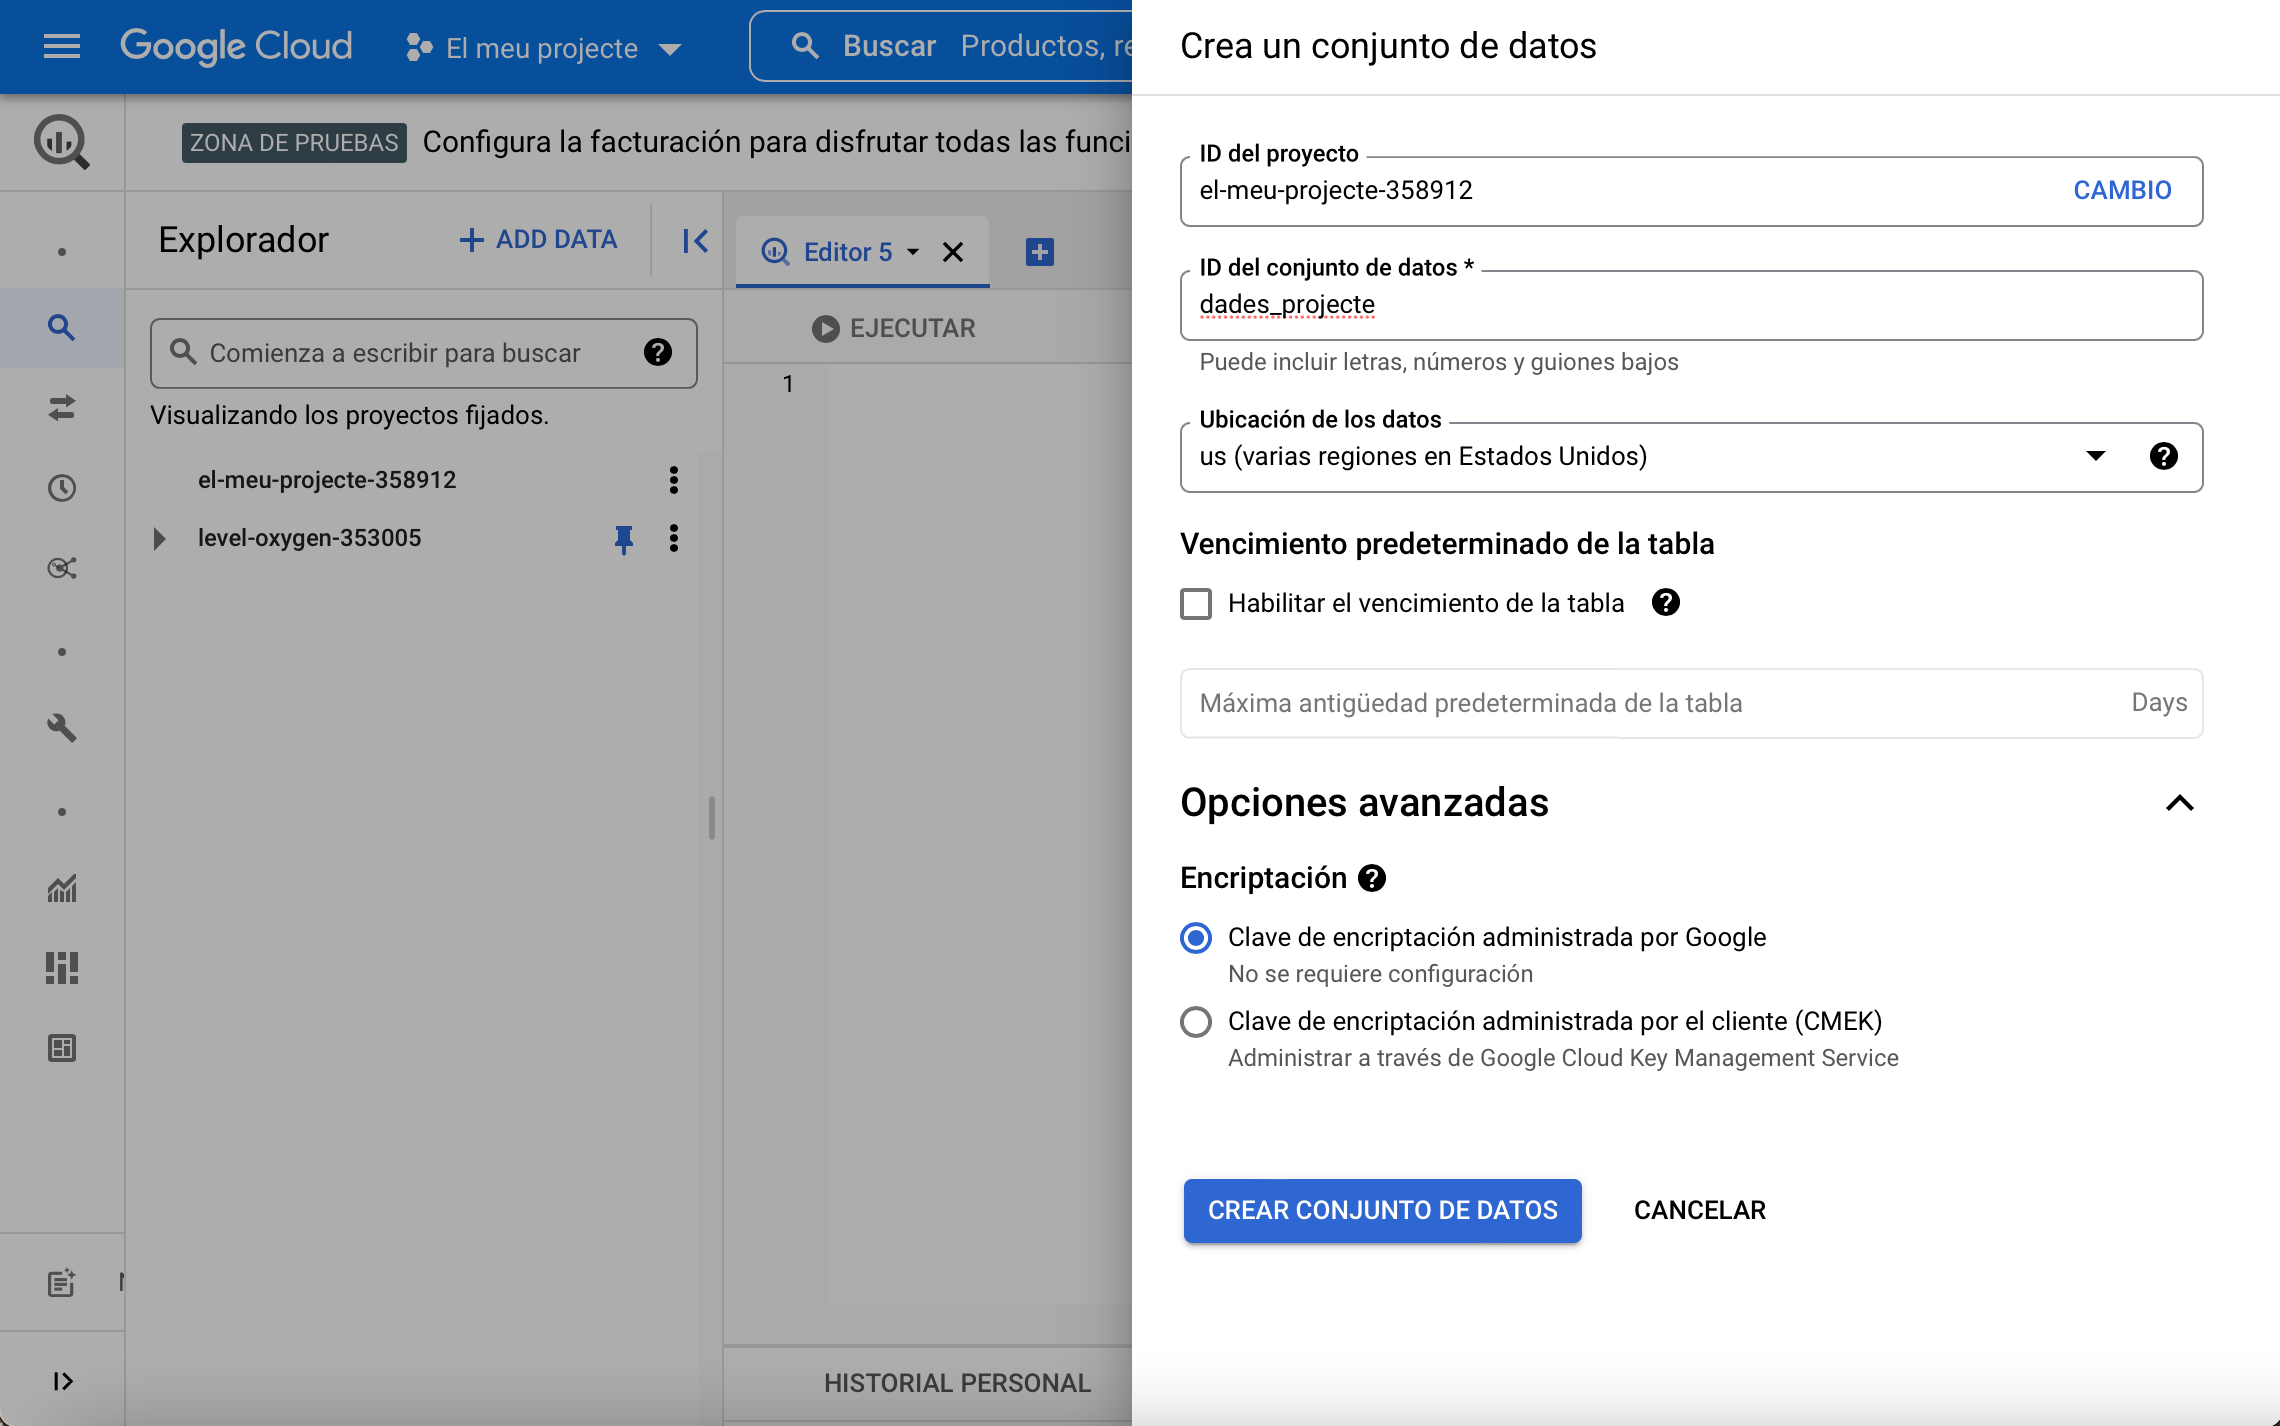
\includegraphics[width=10cm]{bq5}
\end{center}

\vspace{2mm}

Un cop creat, el conjunt de dades \verb|dades_projecte| ara apareix dins de \verb|el_meu_projecte|, I ampliant això s'observa que no hi ha taules dins d'aquest. Ara, es pot donar un cop d'ull als detalls associats a aquest conjunt de dades. Des d'aquest menú, podem triar obrir-lo, moment en el qual la informació del conjunt de dades apareix a la dreta. Aquí podem confirmar l'identificador del conjunt de dades, que també assenyala el projecte en el qual s'ha creat el conjunt de dades, i després altres detalls que inclouen les hores de creació i modificació. 

\vspace{2mm}

A més, des d'aquesta finestra podrem compartir el conjunt de dades amb altres usuaris. Hi ha opcions per a copiar i eliminar aquest conjunt de dades. I després, a \textit{editar detalls}, podem reconfigurar el temps de caducitat de les taules, establir una descripció o afegir etiquetes. Per exemple, si volem marcar aquest conjunt de dades com a pertanyent a un equip, podem establir una etiqueta amb la clau d'equip i el valor corresponent. Després, quan guardem aquest conjunt de dades, les etiquetes apareixen a l'apartat de informació.

\subsection{Definició d'una taula de BigQuery des de la interfície d'usuari}

Després d'haver creat un conjunt de dades en un projecte, ja es pot crear una taula dins d'aquest conjunt de dades. Si tenim la informació del conjunt de dades, hauríem de veure aquesta opció per a crear una nova taula des d'aquí. Alternativament, podem dirigir-nos al projecte, després al conjunt de dades i triar l'opció de crear una taula.

Apareixerà un formulari i tindrem l'opció d'especificar una font per a la nostra taula. Això ens permetrà extreure dades de fonts ja existents, com l'emmagatzematge en el núvol de Google, podríem pujar un arxiu dels nostres propis sistemes d'arxius, i després hi ha un grapat d'altres opcions aquí. La primera taula que crearem serà bastant simple. De fet, serà una taula buida. També existeix l'opció d'establir un tipus de taula. Encara que existeix l'opció d'establir una taula, per a emmagatzemar les seves dades fora de BigQuery, notaràs que no està disponible per a una taula buida, cosa que significa que les nostres dades seran natives del servei BigQuery. A continuació, passem a la secció d'Esquema. Podem especificar l'esquema com a text o podem fer ús d'aquesta interfície per a establir les columnes de la nostra taula, incloent-hi els tipus i altres configuracions. La primera columna que definiré és l'ANEU de l'alumne. Per al tipus, podem triar d'un menú, que inclou tots els tipus amb els quals potser ja estàs familiaritzat. Quant a la manera, aquest determinarà si els valors d'aquesta columna poden ser nuls, és a dir, si són anul·lables o si es requereix un valor. També podem establir que els valors siguin d'un tipus repetit com (indistint). També podem establir una descripció, que és opcional, i amb la primera columna definida, passem a la columna número dos. L'altra opció a l'hora d'especificar l'esquema d'una taula és definir-lo en forma de text. Notaràs que el format aquí és molt semblant a JSON i podem especificar el nom, tipus, manera, així com altres propietats per a cada camp. La versió de text de l'esquema també pot ser útil si vols guardar-ho en algun sistema de control de versions.

Seguim endavant, llavors. També podem configurar el particionamiento d'una taula, que determinarà com es divideixen les seves dades en l'emmagatzematge. La partició pot fer-se sobre la base del temps d'ingestió o sobre la base d'un camp sencer o de data. També podem especificar com agrupar les nostres dades.

\subsubsection{Afegir dades a una taula de BigQuery senzilla}

Ara que hem creat una gran taula de consulta, podem centrar-nos en treballar amb ella. Per a això, bo, primer, ens desplaçarem cap avall aquí, i donar un cop d'ull al primer esquema de la taula. En algun moment de la seva vida, és possible que necessitis editar l'esquema, la qual cosa pots fer prement aquest botó, i després fent els canvis necessaris. Podries canviar les propietats dels camps existents o podries afegir altres nous. Jo deixo les coses com estan, i surto d'aquesta vista, i després passem als detalls de la taula. I aquí és on podem donar un cop d'ull a alguna informació interessant. Més enllà de la identificació de la taula, també podem comprovar la grandària de la taula, que ens donarà una indicació de la quantitat de dades que es processaran, si anéssim a executar consultes contra ella. La grandària d'emmagatzematge a llarg termini assenyala les dades als quals no s'ha accedit en els últims 90 dies, i després, per descomptat, tenim les hores de creació i modificació juntament amb la ubicació de les dades de la taula, que correspon a la ubicació de l'alimentador de dades que va ser reemplaçat. Des d'aquesta interfície, també podem editar els detalls existents d'aquesta taula. Aquí podem establir un temps de caducitat en cas que vulguem anul·lar el que s'ha establert en el nivell del conjunt de dades. També tenim l'opció d'establir una descripció o afegir etiquetes.

Això ens donarà un cop d'ull a les dades de la taula, i com és lògic, aquí no hi ha dades. Canviarem això i inserir una nova fila de dades per a això ens dirigim a compondre una nova consulta. Des de la interfície que apareix, podem pegar la consulta que necessitem executar. Comencem amb "insert into", seguit de la taula en la qual s'ha de realitzar la inserció. Per a això, utilitzem parèntesi, i dins dels parèntesis, utilitzem la sintaxi, data set *name *dot *able *name, que en el meu cas és, *loony* underscore university.students. A continuació, en la línia número dos, podem especificar els noms de les columnes per a les quals s'afegiran valors, així que, com s'ha especificat, cadascuna de les cinc columnes presents en la taula, i després, seguit de la paraula clau values, especifiquem entre parèntesi, els propis valors. Observi's que en les consultes grans, podem utilitzar cometes dobles en especificar cadenes. També hi ha una altra informació interessant aquí per a la que minimitzaré el panell de l'explorador. Notaràs que hi ha un missatge que assenyala que es processaran zero bytes, quan executem aquesta consulta. Ara, seguirem endavant i executar aquesta consulta, i sembla que la inserció va ser un èxit, atès que una fila s'ha afegit a la taula dels estudiants. Per a confirmar-ho, executem una consulta més, concretament, un select from loony university.students. Significativament, obtenim un missatge que diu que, en executar aquesta consulta, es processaran 60 bytes de dades, assenyalant el cost que es produirà. Efectivament, l'única fila ha estat retornada, i fins i tot en els resultats de la consulta, obtenim la confirmació que s'han processat 60 bytes. El temps d'execució de la consulta també apareix aquí.

\subsection{Càrrega de dades per crear una taula de BigQuery}

Mentre que anteriorment vam veure com podem crear una taula buida i després emplenar-la amb dades amb sentències INSERT, ara explorarem un cas d'ús més comú per als usuaris de BigQuery en el qual es crea una taula a partir de dades existents. Per a això, ens dirigirem al conjunt de dades $loony_university$ i triarem crear una nova taula. I aquesta vegada, la font no serà una taula buida, sinó que carregarem un arxiu CSV del nostre propi sistema d'arxius per al qual es pot seleccionar l'opció de càrrega. Hi ha algunes restriccions quant a la grandària de l'arxiu que podem pujar. Per tant, aquest ha de romandre dins dels 100 MB. No obstant això, per als arxius més grans, encara podem portar-los a BigQuery, sempre que els moguem en l'emmagatzematge en el núvol de Google primer. Procedim llavors a navegar pels nostres sistemes d'arxius per a l'arxiu a pujar. I després navegar fins a $movies_info.csv$. Aquest arxiu està inclòs en els materials del curs. També es pot descarregar des d'aquesta ubicació. Una vegada que l'arxiu ha estat seleccionat. I després obert. Sabrà que el format de l'arxiu s'ha establert automàticament en CSV. Perquè et facis una idea, alguns dels altres formats suportats aquí inclouen JSON així com Avro. Quant al projecte i al conjunt de dades, els deixarem com estan. I després, el nom de la taula, $movies_info$, transmetrà que sí que inclou informació sobre diverses pel·lícules. A continuació, tenim l'opció de definir explícitament l'esquema. No obstant això, atès que es tracta d'un arxiu CSV amb múltiples columnes, podem triar l'opció Acte detectar. Aquí, BigQuery donarà un cop d'ull al contingut de cada columna i determinarà quin ha de ser l'esquema. Més enllà d'això, deixem tota la resta sense tocar. I després, tria crear la taula. En uns moments, notaràs que $movies_*nfo$ apareix sota el conjunt de dades $loony_university$. En cas que no ho vegis, és possible que hagis d'actualitzar la pàgina en el teu navegador. A continuació, podem accedir a la informació de la taula i al seu contingut desplegant el menú i triant Obrir. En l'esquema de la taula, sabrà que s'ha detectat automàticament el tipus dels diferents camps. El nom de la productora, el país en el qual es troba, així com els noms dels directors s'especifiquen com a cadenes, però el pressupost s'ha detectat i establert com un nombre enter. Si continuem avançant, observarem que la columna de puntuació s'ha configurat com un valor de coma flotant. I tenim un grapat d'uns altres en enters i cadenes en l'esquema. Donem un cop d'ull als detalls de la taula. Aquí notaràs que la grandària total és de poc més de 720 KB. El nombre de files és d'unes 4.600. I després, quan ens dirigim a la Vista Prèvia, bo, aquí és on obtenim un cop d'ull als continguts. Efectivament, la columna del pressupost és un nombre enter bastant gran. Igual que el tipus d'aquesta columna, el conjunt de dades inclou el nom de l'empresa o de l'estudi que ha produït la pel·lícula. També tenim aquí la informació del director. El gènere de la pel·lícula. I després, desplaçant-se al llarg, el nom o títol de la pel·lícula, juntament amb els diners que va tancar en la taquilla. I després, podem desplaçar-nos més a baix per a donar un cop d'ull a les pel·lícules que són presents en aquest conjunt de dades.

\subsection{Consulta de dades i visualització d'estadístiques de consultes}

\subsection{Creació d'una taula a partir d'un resultat de consulta}

\subsection{Creació d'una consulta a partir d'un filtre}

\newpage

\section{Execució de consultes i visualització de resultats}

\subsection{Conjunts de dades públics a BigQuery}

\subsection{Configuració i ús de memòria cau de BigQuery}

\subsection{Taules externes de BigQuery}

\subsection{Integració de BigQuery amb Data Studio}

\newpage


\end{document}
